
\subsection{Wizard Design}

TUG Wizard is a wizard-like application that helps developers create and
configure test projects to test Qt based panels and their related classes.
%
Its architecture design is depicted in the figure below.

\vspace{2ex}
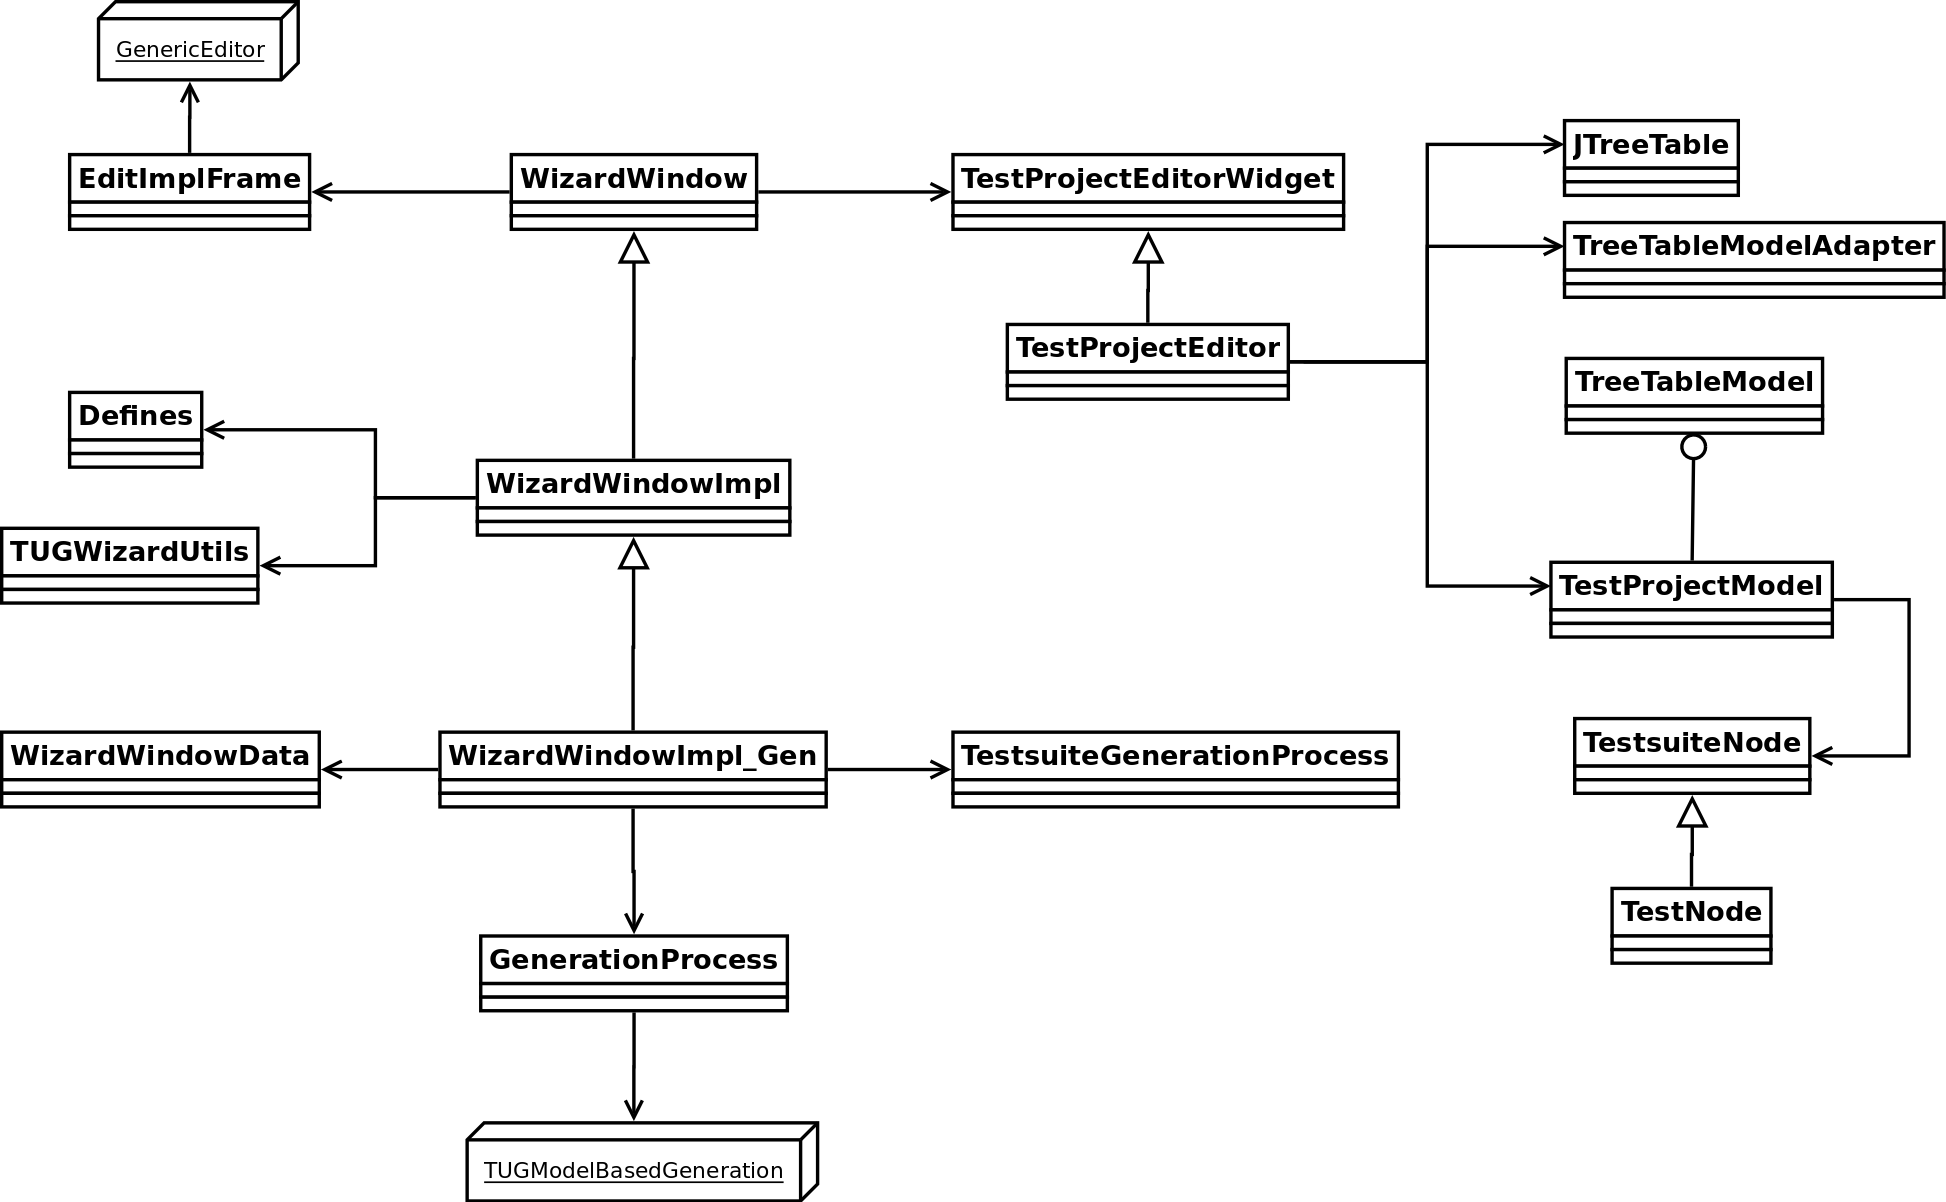
\includegraphics[width=.99\textwidth]{images/diag/tug_wizard_classdiag.png}
\vspace{2ex}

This architecture is divided into three levels. Inheritance is used to
divide the implementation of {\tt WizardWindow} into the following three
classes:
%
\begin{itemize}
\item {\tt WizardWindow}: includes configuration and deployment of TUG
  Wizard user interface.
%
\item {\tt WizardWindowImpl}: includes the implementation under the TUG
  Wizard user interface, excluding generation functionality.
%
\item {\tt WizardWindowImpl\_Gen}: includes the implementation of the
  test project generation processes.
\end{itemize}

The most relevant classes included at each of these levels are further
described in the following.

\newpage

%%%
%%% WizardWindow

As said above, \field{WizardWindow} implements the configuration and
deployment of TUG Wizard user interface. It uses two supporting classes,
\field{EditImplFrame} and \field{TestProjectEditorWidget}, used to allow
developers to edit configuration files and to configure a test project
structure, respectively.  


\field{EditImplFrame} is the main class of \field{GenericEditor}, an
external component used in TUG Wizard in Steps 4 and 5 to allow the
modification of configuration files. This component is not further
described because it is out of the scope of this guide.


\vspace{2ex}
\begin{center}
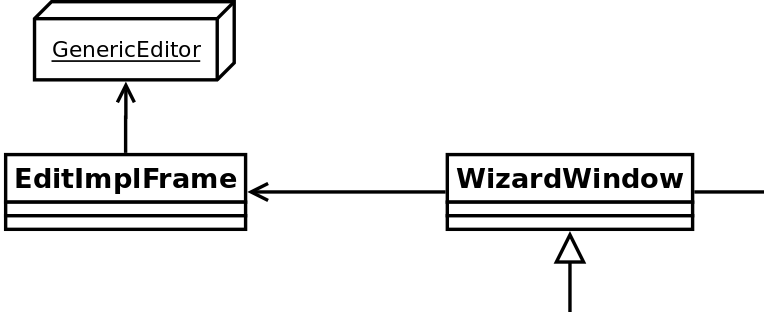
\includegraphics[width=.65\textwidth]{images/diag/tug_wizard_classdiag_ww1.png}
\end{center}
\vspace{2ex}


\field{TestProjectEditorWidget} represents the component to configure a
test project structure composed of a set of testsuites and tests (Step 6 in
TUG Wizard). The editor is based on a \field{JTreeTable} object and uses an
underlying model described by \field{TestProjectModel}.


\vspace{2ex}
\begin{center}
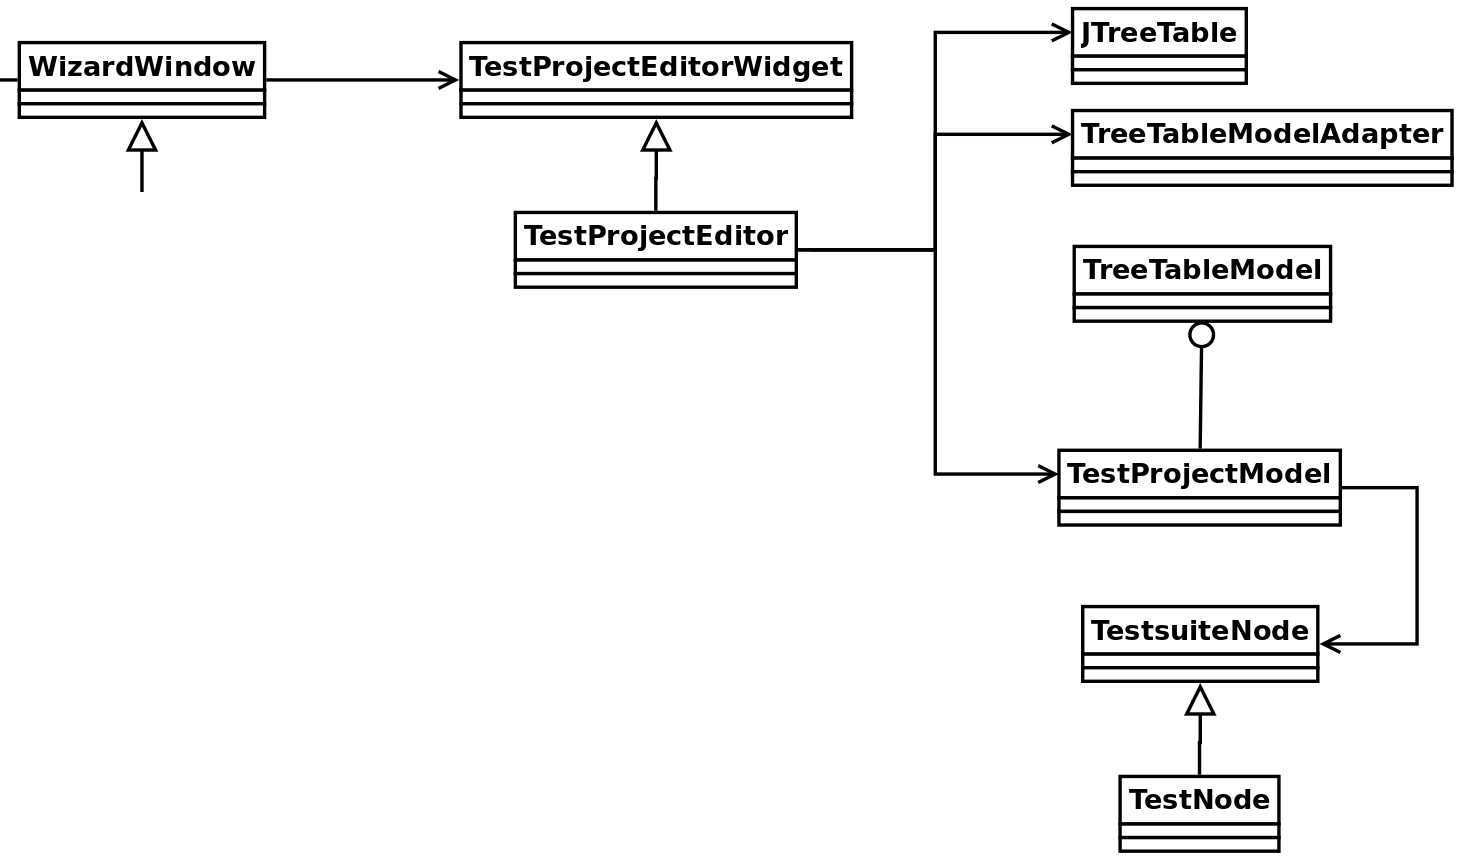
\includegraphics[width=.99\textwidth]{images/diag/tug_wizard_classdiag_ww2.png}
\end{center}
\vspace{2ex}


%%%
%%% WizardWindowImpl

\field{WizardWindowImpl} includes all the implementation under the TUG
Wizard user interface. It implements all steps in the process, excluding
Step 7 in which the generation process is carried out.

\field{TUGWizardUtils} implements supporting methods to simplify the wizard
processes.
%
The \field{Defines} class defines some constant values used during the
wizard and generation processes.


\vspace{2ex}
\begin{center}
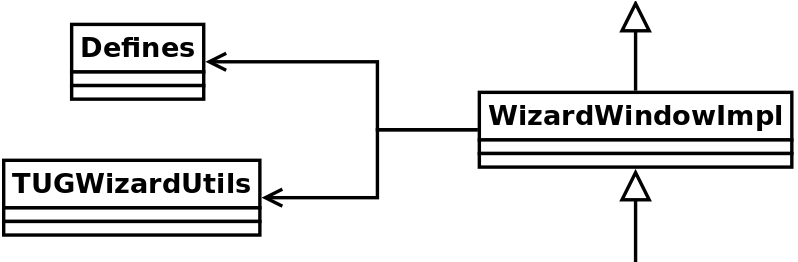
\includegraphics[width=.65\textwidth]{images/diag/tug_wizard_classdiag_wwi1.png}
\end{center}
\vspace{2ex}


%%%
%%% WizardWindowImpl\_Gen

\field{WizardWindowImpl\_Gen} includes all the implementation of the TUG
Wizard related to the test project generation processes. 


\vspace{2ex}
\begin{center}
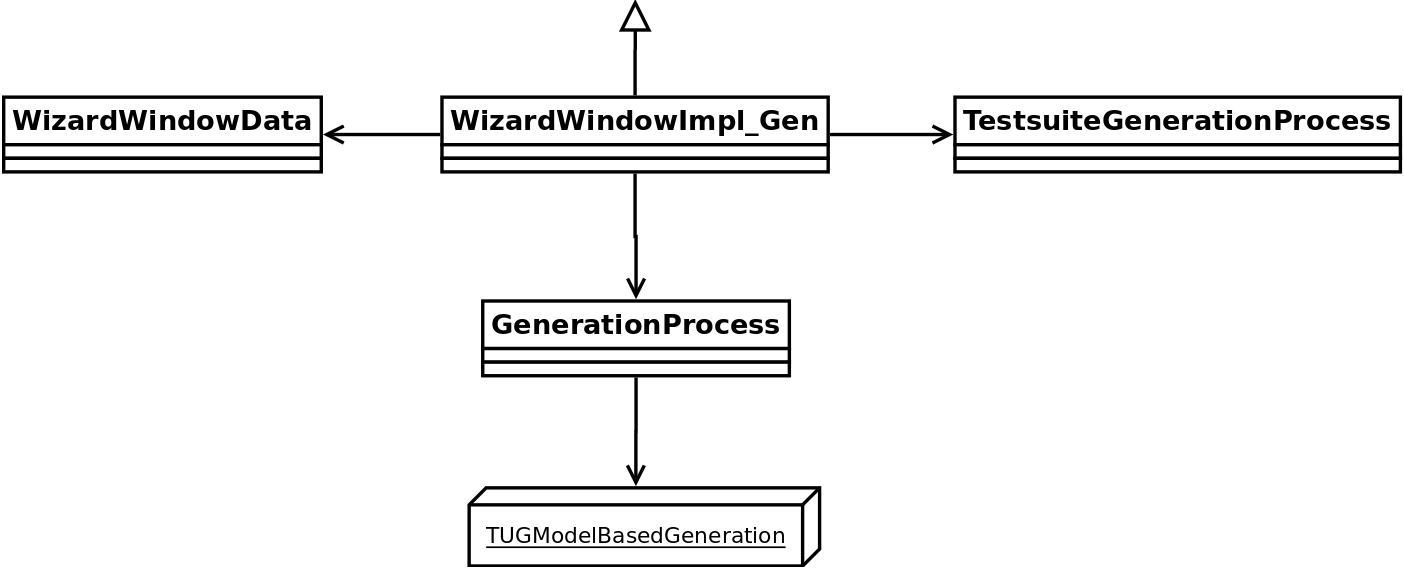
\includegraphics[width=.99\textwidth]{images/diag/tug_wizard_classdiag_wwig1.png}
\end{center}
\vspace{2ex}


The generation processes are based on the data encapsulated within
\field{WizardWindowData}. This object includes all configuration data
provided by developers during the wizard steps.


%%%
\field{GenerationProcess} encapsulates the generation of a new test panel
project. This process uses the Qt panel and the dependencies introduced by
developers in the wizard steps to generate a new panel to be tested.
%
This new panel inherits the original one and includes methods to simulate
users interaction with the widgets composing the panel. These methods are
aimed at being used in tests definition.
%
It is also generated a Qt project to compile and run this panel standalone.


%%%
The \field{TestsuiteGenerationProcess} class includes methods supporting
the generation of a test project structure. A test project is composed of:
%
\begin{itemize}
\item a main project called {\tt build\_all.pro} from which everything can
  be compiled.
\item the test panel project described above. It is included in {\tt
  \_main} folder. 
\item a set of testsuites. Each testsuite includes a set of empty methods
  (i.e., the tests) to be filled by developers with the desired
  functionality. Methods from the test panel and from {\tt qt\_TestUtils}
  class can be used to support the tests implementation.
\item a Qt project for each testsuite. This project can be used to compile
  and run the testsuites standalone.
\end{itemize}



%%%
%%%


%\begin{lstlisting}
%xxxx
%\end{lstlisting}



\newpage


%%% Local variables:
%%% mode: latex
%%% TeX-master: "README.tex"
%%% ispell-local-dictionary: "american"
%%% coding: utf-8
%%% fill-column: 75
%%% TeX-parse-self: t
%%% TeX-auto-save: t
%%% End:
